\documentclass[12pt]{extarticle}

%%%%%%% PACKAGES %%%%%%%%
\usepackage[utf8]{inputenc}
\usepackage[margin=2.5cm]{geometry}
\usepackage{blindtext}
\usepackage{setspace}
\usepackage{graphics}
%\usepackage{epstopdf}
\usepackage{notoccite} %citation number ordering
\usepackage{lscape} %landscape table
\usepackage{caption} %add a newline in the table caption
\usepackage{hyperref}
\usepackage{enumitem}
\usepackage{datetime}
\usepackage{titlesec}
\usepackage{booktabs} % For \toprule, \midrule and \bottomrule
\usepackage{siunitx} % Formats the units and values
\usepackage{pgfplotstable} % Generates table from .csv
\usepackage{amsmath}
\usepackage{bm}

\usepackage{chngcntr}
\counterwithin{figure}{section}
\titleformat*{\section}{\LARGE\bfseries}
\titleformat*{\subsection}{\Large\bfseries}
\titleformat*{\subsubsection}{\large\bfseries}

\newdateformat{monthyeardate}{%
	\monthname[\THEMONTH], \THEYEAR}

\onehalfspace   % 1.5 line spacing

\title{
\includegraphics[width=4cm]{pics/AAU_Logo.jpg}\\\Large{\textbf{Breast Cancer and Benign Detection using Hierarchical Deep Convolutional Neural Networks}}
\date{}}
\begin{document}
	\clearpage\maketitle
	\begin{center}
		\vspace{-1.5cm}
		\large{\emph{Submitted by}}\\\vspace{0.5cm}
		\begin{tabular}{l l}
			
			\multicolumn{1}{p{6cm}}{ \large{\textbf{Yacoub Abu Lubad}}} &  \multicolumn{1}{p{6cm}}{\centering \large{\textbf{201930007}}} 
		\end{tabular}\\\vspace{1cm}
		\large{\emph{Supervised by}}\\\vspace{0.5cm}
		\large{\textbf{Assistant Prof. Dr. Talal A. Edwan}}\\\vspace{1cm}
		{Submitted in partial fulfillment of the requirements for the award of the Bachelor of Science in Computer Engineering Degree\\\vspace{1cm}
		Faculty of Engineering\\Al-Ahliyya Amman University\\Amman - Jordan}\\ \vspace{0.5cm}
		\Large{\textbf{\monthyeardate\today}}
		\pagenumbering{roman} % Start roman numbering
		
		\thispagestyle{empty}
	\end{center}
	\newpage
	% % Start roman numbering
	\setcounter{page}{1}
	%%% CONTENT HERE %%%%
	\begin{center}
	\Large{\textbf{Acknowledgments}}\\ \vspace{1cm}
	\end{center}
	Acknowledgment Goes Here...
	\newpage
	
	\tableofcontents
	\listoffigures
	\listoftables
	\newpage
	\begin{center}
		\LARGE{\textbf{Descriptive Abstract}}\\ \vspace{1cm}
	\end{center}
	Abstract goes here...\\
	Keywords: \emph{Keyword1, Keyword2, ... , Keywordn}
	\newpage
	\LARGE{\textbf{List of Abbreviations}}\\ \vspace{1cm}
	\begin{center}
		\begin{tabular}{l l}
			\multicolumn{1}{p{3cm}}{\large{\textbf{AI}}} &  \multicolumn{1}{p{8cm}}{\large{\textbf{A}rtificial \textbf{I}ntelligence}} \\
			\multicolumn{1}{p{3cm}}{\large{\textbf{ANN}}} &  \multicolumn{1}{p{8cm}}{\large{\textbf{A}rtificial \textbf{N}eural \textbf{N}etwork}} \\
			\multicolumn{1}{p{3cm}}{\large{\textbf{CNN}}} &  \multicolumn{1}{p{8cm}}{\large{\textbf{C}onvolutional \textbf{N}eural \textbf{N}etwork}}\\ 
			\multicolumn{1}{p{3cm}}{\large{\textbf{GPU}}} &  \multicolumn{1}{p{8cm}}{\large{\textbf{G}raphical \textbf{P}rpcessing \textbf{U}nit}}\\ 
			\multicolumn{1}{p{3cm}}{\large{\textbf{HD-CNN}}} &  \multicolumn{1}{p{8cm}}{\large{\textbf{H}ierarchical \textbf{D}eep \textbf{C}onvolutional \textbf{N}eural \textbf{N}etwork}}\\ 
			\multicolumn{1}{p{3cm}}{\large{\textbf{MAE}}} &  \multicolumn{1}{p{8cm}}{\large{\textbf{M}ean \textbf{A}bsolute \textbf{E}rror}}\\  
			\multicolumn{1}{p{3cm}}{\large{\textbf{MLP}}} &  \multicolumn{1}{p{8cm}}{\large{\textbf{M}ulti\textbf{l}ayer \textbf{P}erceptron}}\\ 
			\multicolumn{1}{p{3cm}}{\large{\textbf{CNN}}} &  \multicolumn{1}{p{8cm}}{\large{\textbf{C}onvolutional \textbf{N}eural \textbf{N}etwork}}\\ 
			\multicolumn{1}{p{3cm}}{\large{\textbf{CNN}}} &  \multicolumn{1}{p{8cm}}{\large{\textbf{C}onvolutional \textbf{N}eural \textbf{N}etwork}}\\ 
			\multicolumn{1}{p{3cm}}{\large{\textbf{CNN}}} &  \multicolumn{1}{p{8cm}}{\large{\textbf{C}onvolutional \textbf{N}eural \textbf{N}etwork}}\\
			\multicolumn{1}{p{3cm}}{\large{\textbf{HDD}}} &  \multicolumn{1}{p{8cm}}{\large{\textbf{H}ard \textbf{D}isk \textbf{D}rive}}\\ 
			\multicolumn{1}{p{3cm}}{\large{\textbf{RAM}}} &  \multicolumn{1}{p{8cm}}{\large{\textbf{R}andom \textbf{A}ccess \textbf{M}emory}}
			 
		\end{tabular}
	\end{center}

	\newpage
	\LARGE{\textbf{List of Symbols}}\\ \vspace{1cm}
	\large{}
	\begin{center}
		\begin{tabular}{l l}
			{Symbol} & {Name} \\
			$b$ & bias\\
			$w$ & weights\\
			$\phi$ & activation function\\
			$\eta$ & cost function
		\end{tabular}
	\end{center}
	
	
	\newpage
	\large{}
	\pagenumbering{arabic}
	\section{Introduction}
	The \emph{motivation} of this Thesis will be discussed in Section \ref{Motiv}, while explaining more what the \emph{actual problem} is and the \emph{purpose of this Thesis} in Section \ref{delay problem}. As for the \emph{objectives} of this Thesis, that will be briefly discussed in Section \ref{Obj}, while the \emph{organization} and the structure of this Thesis is to be discussed in Section \ref{Org}.
	\subsection{Motivation}\label{Motiv}
	
	Breast cancer is the most common cause of new cancer cases, according to the \textbf{World Health Organization (WHO)}, standing at 2.26 million recorded cases in 2020, meanwhile, the total count of cancer caused mortality cases are recorded to be 10 million in 2020, breast cancer is documented to have caused 685,000 deaths in 2020 \cite{WHO_stats}. There are multiple ways of reducing the mortality rate of this disease, one of the main approaches would be early detection. A study has proved that a delayed diagnosis and detection of \emph{more than 6 weeks} gave these cancerous cells enough time to develop into much dangerous stages, but diagnosis that were conducted \emph{under 6 weeks} of delay detected less advanced stages of these cells \cite{caplan2014delay}. So the earlier the detection of these cells are prompted, the safer and less severe it is on the patient.
	\\[5mm]
	This sort of detection is done via Screening Mammography where a patient undergoes 4 different kinds x-ray imaging, one image is taken from the side of the breast and the second is from the top, same procedure is repeated on the second breast \cite{healthline}. This totals in 4 images per patient where the radiologist can evaluate whether there are any \emph{abnormalities} detected, which are usually \emph{lumps} that are classified into two categories, \emph{Benign and Cancer}. The only downfall is that if any abnormalities are detecting after the first evaluation, the patient is contacted, which could typically take up to a week or two, to visit and perform a diagnostics test so that the abnormality could be studied even further in classifying whether it is cancerous or not \cite{healthline}.\\[5mm]
	
	\subsubsection{The result delay problem}\label{delay problem}
	As discussed in Section~\ref{Motiv}, the issues of late diagnosis and detection of these cancerous cells would increase the mortality rate, and it has also been pointed out that the results of any abnormalities detected by the radiologist could only be known after a duration of week or two. This problem can be tackled by reducing the time of detecting the abnormalities from \emph{1-2 weeks} all the way down to matter of \textbf{fractions of a second.}\\[5mm]
	This method is a great aid in early detection, this way the patient would have a time advantage to proceed to the diagnosis of this abnormality right away. However, it is also possible to \emph{skip} the diagnosis procedure as well, saving even more time when all it would require is one mammography screening and the results would be ready the moment the screening is completed.\\[5mm]
	A key feature in making this quick and accurate detection is using two methods that fall under the \textbf{Artificial Intelligence (AI)} domain, \emph{Image Classification} and \emph{Object Detection}.
	
	\subsection{Objectives}\label{Obj}
	The goal of this thesis is to compare and contrast the different results that could be obtained using different \emph{Convolutional Neural Network (CNN)} model structures. Applying \textbf{4 different concepts} to the same dataset but with different utilization of the data to measure the accuracy that might be obtained when manipulating the data differently. Due to the vast dataset that was obtained, one of the multiple hardware constraints were during loading the images from the \emph{Hard Disk Drive (HDD)} onto the \emph{Random Access Memory (RAM)}, there was no enough memory to load the whole dataset to proceed with the model training. \\[5mm]
	A different kind of hardware constraint that was faced is the absence of \emph{Graphical Processing Unit} (GPU), a GPU is crucial for \emph{Computer Vision} (CV) due to the enormous data stream that will take place during training \cite{GPU} \cite{GPU}.
	\subsection{Organization}\label{Org}
	The \emph{Literature Review} will be discussed in \emph{Section~\ref{Lit. Rev.}} alongside the essential background on the different kinds of Neural Networks with their diverse functionalities. A deeper dive into the application's functions will be thoroughly described in \emph{Section~\ref{CV}} and the two main techniques that will be implemented in this Thesis. In \emph{Section~\ref{Meth}}, there will be a detailed explanation on the \textbf{Hierarchical approach} that is applied to obtain the results as well as the methods that helped surpassed the constraints that were mentioned in \emph{Secion~\ref{Obj}}. Detailed dissection of the dataset will be in \emph{Section~\ref{Data}}.
	\newpage
	\section{Background}\label{Lit. Rev.}
	This thesis will focus on implementing a \emph{Hierarchical Object Detector with Classifier}. There has been previous implementations of Brest cancer detection using a \emph{one stage} object detection, which will be explained in \emph{Section~\ref{Obj Detection}}, as seen in \cite{one_shot}, but the gap remains with setting up a \emph{two stage} object detector to detect and classify these tumors. In other words, this is an application of \textbf{Hierarchical Deep Convolutional Neural Network} since it relies on \emph{Hierarchy}, which will be explained in \emph{Section~\ref{Meth}}.
	\subsection{Artificial Neural Networks}\label{ANN}
	\emph{Artificial Neural Networks (ANNs)} are a simplified mathematical models that mimic the functionality of a human brain and nervous system \cite{ANN, ANN2}. Just like humans, these networks were designed to solve more complex, \emph{non-linear}, highly stochastic and multi-variable problems that a traditional program could not. These problems span out to the fields of medicine, finance, security and many more \cite{ANN_funct}. \emph{ANNs} are designed to approximating any continuous function thus are used in a wide spectrum of applications such as object detection \cite{Objdet, Objdet2}, image classification \cite{classification}, image enhancement \cite{enhancement} as well as several more uses.\\[5mm]
	The \emph{ANN} is originally compromised from multiple \emph{neurons}, or \emph{perceptron}, which can be demonstrated in \emph{Figure~\ref{fig:Perceptron}}, hence the \emph{perceptron} is the ground foundation of \emph{ANNs}.
	\begin{figure}[h]
		\centering
		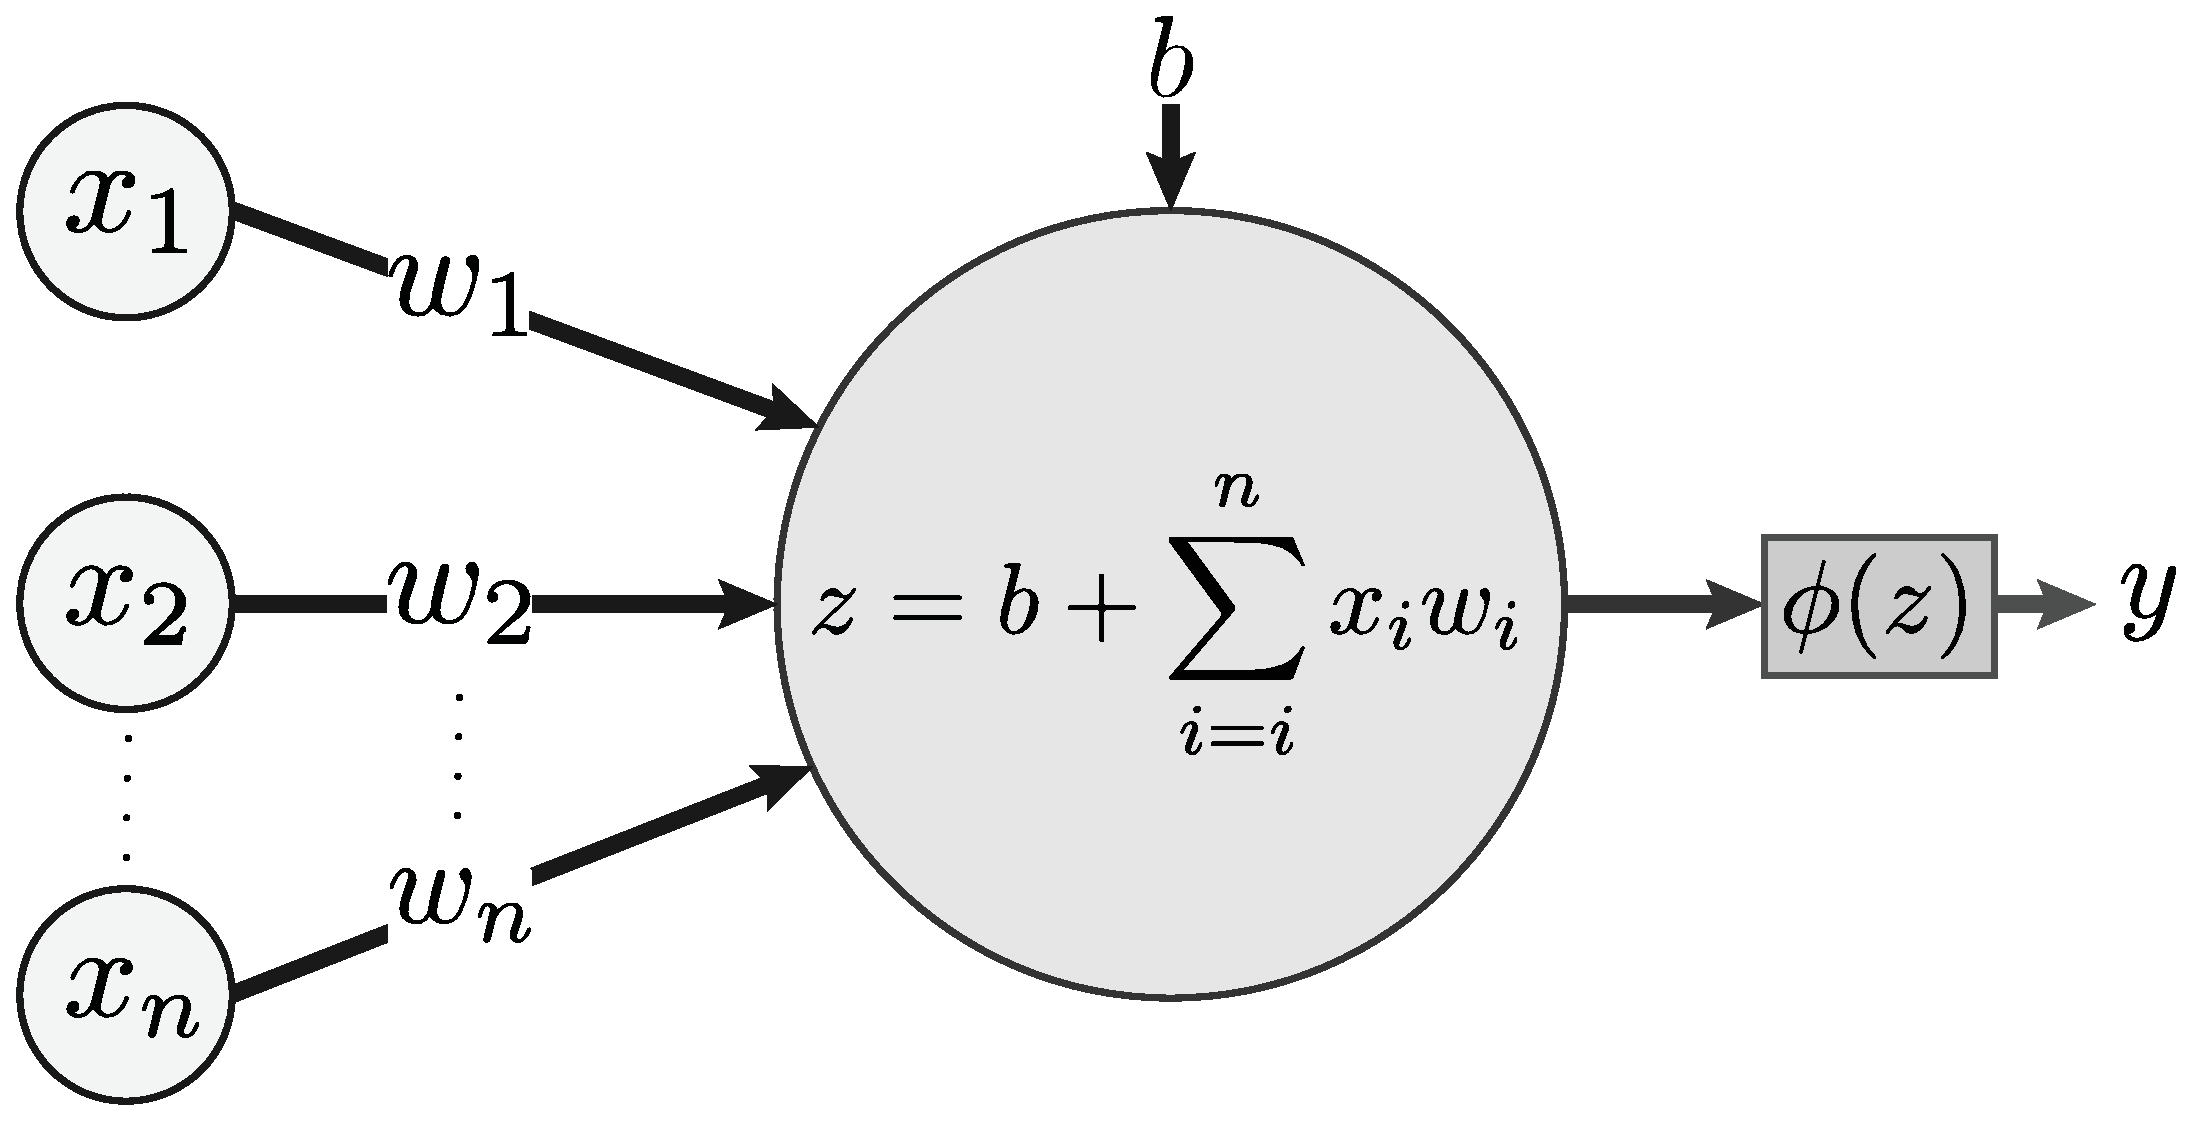
\includegraphics[width=0.7\textwidth]{pics/Figures/Perceptron.eps}
		\caption{\small{Artificial Neuron \emph{(Perceptron)}}}
		\label{fig:Perceptron}
	\end{figure}
	
	The input $\bm{x}$ of size $\bm{n}$ for this perceptron is denoted as the input vector that is composed of numerical values representing different features of a single entry as seen below.
	\begin{align}
	\bm{x} &= \begin{bmatrix}\label{inputs}
		x_1 \\
		x_2 \\
		\vdots \\
		x_n
	\end{bmatrix}
	\end{align}

	Depending on the features of a given model data, different features require different \emph{weights}, denoted as $\bm{w}$, since one feature would have more effect on the final output more than a different kind of feature, thus an input must be multiplied with a weight to determine its importance to the final output.
	\begin{align}
		\bm{w} &= \begin{bmatrix}\label{weights}
			w_1 \quad
			w_2 \quad
			\cdots \quad
			w_n
		\end{bmatrix}
	\end{align}
	
	The above vector will differ based on the next layer's size, given that there is $\bm{m}$ number of neurons in the next layer, the \emph{weight's matrix} will have a size of $\bm{m \times n}$ as seen in \emph{Equation~\ref{weights_expanded}}. The weight vector is a \emph{row vector} due to the relationship it contains with the input as every $\bm{n^{th}}$ input, there's a $\bm{n^{th}}$ weight corresponding to it.\\[5mm]
	After the input is multiplied with its assigned weight, it is now referred to as the \textbf{weighted input}, that weighted input is summed with the rest of the weighted inputs which then derives us the \textbf{weighted sum}. Then as all these inputs are summed, a \emph{bias} $\bm{b}$ is added which is an additional parameter that is used to adjust the \emph{output} of the perceptron as well as the weighted sum that is \emph{inputted} into the perceptron.\\[5mm]
	\newpage
	The output of the perceptron can be denoted as $\bm{y}$ and is calculated as follows:
	\begin{equation}\label{output}
		y = \phi{(z)},
	\end{equation}
	where
	\begin{equation}\label{z}
		z = b + \sum_{i}^{n} x_i w_i
	\end{equation}
	
	The $\phi$ is an arbitrary function known as the \textbf{activation function} \cite{agarap2018deep} 
	%Talk about relu
	%
	%
	which is responsible for causing the perceptron to \emph{fire} generating an output. This activation function is deduced by a threshold that is set based on the different types of activation functions alongside their different uses which can limit the output of reaching an undesired or unacceptable value \cite{siddique2013computational}.\\[5mm]
	
	The expansion from a single perceptron to multi perceptrons forms a \emph{single layered neural network} as seen in \emph{Figure~\ref{fig:ANN}}; using the input vector as seen in \emph{Equation \ref{inputs}} and defining the weights matrix 
	\begin{align}
		 W &= \begin{bmatrix}\label{weights_expanded}
			w_{1,1}\quad w_{1,2} \quad \cdots \quad w_{1,n}\\
			w_{2,1} \quad w_{2,2} \quad \cdots \quad w_{2,n}\\
			\vdots \qquad \vdots \qquad \ddots \qquad \vdots\\
			w_{m,1} \quad w_{m,2} \quad \cdots \quad w_{m,n}
		\end{bmatrix}
	\end{align}
	where $\bm{m}$ is the number of perceptrons and $\bm{n}$ is the number of inputs. The weight responsible for the $\bm{n^{th}}$ input and $\bm{m^{th}}$ perceptron is written as $\bm{w_{m,n}}$. While the bias vector is defined as:
	\begin{align}
		\bm{b} &= \begin{bmatrix}\label{bias_vector}
			b_1 \\
			b_2 \\
			\vdots \\
			b_m
		\end{bmatrix}
	\end{align}

	\begin{figure}[h]
	\centering
	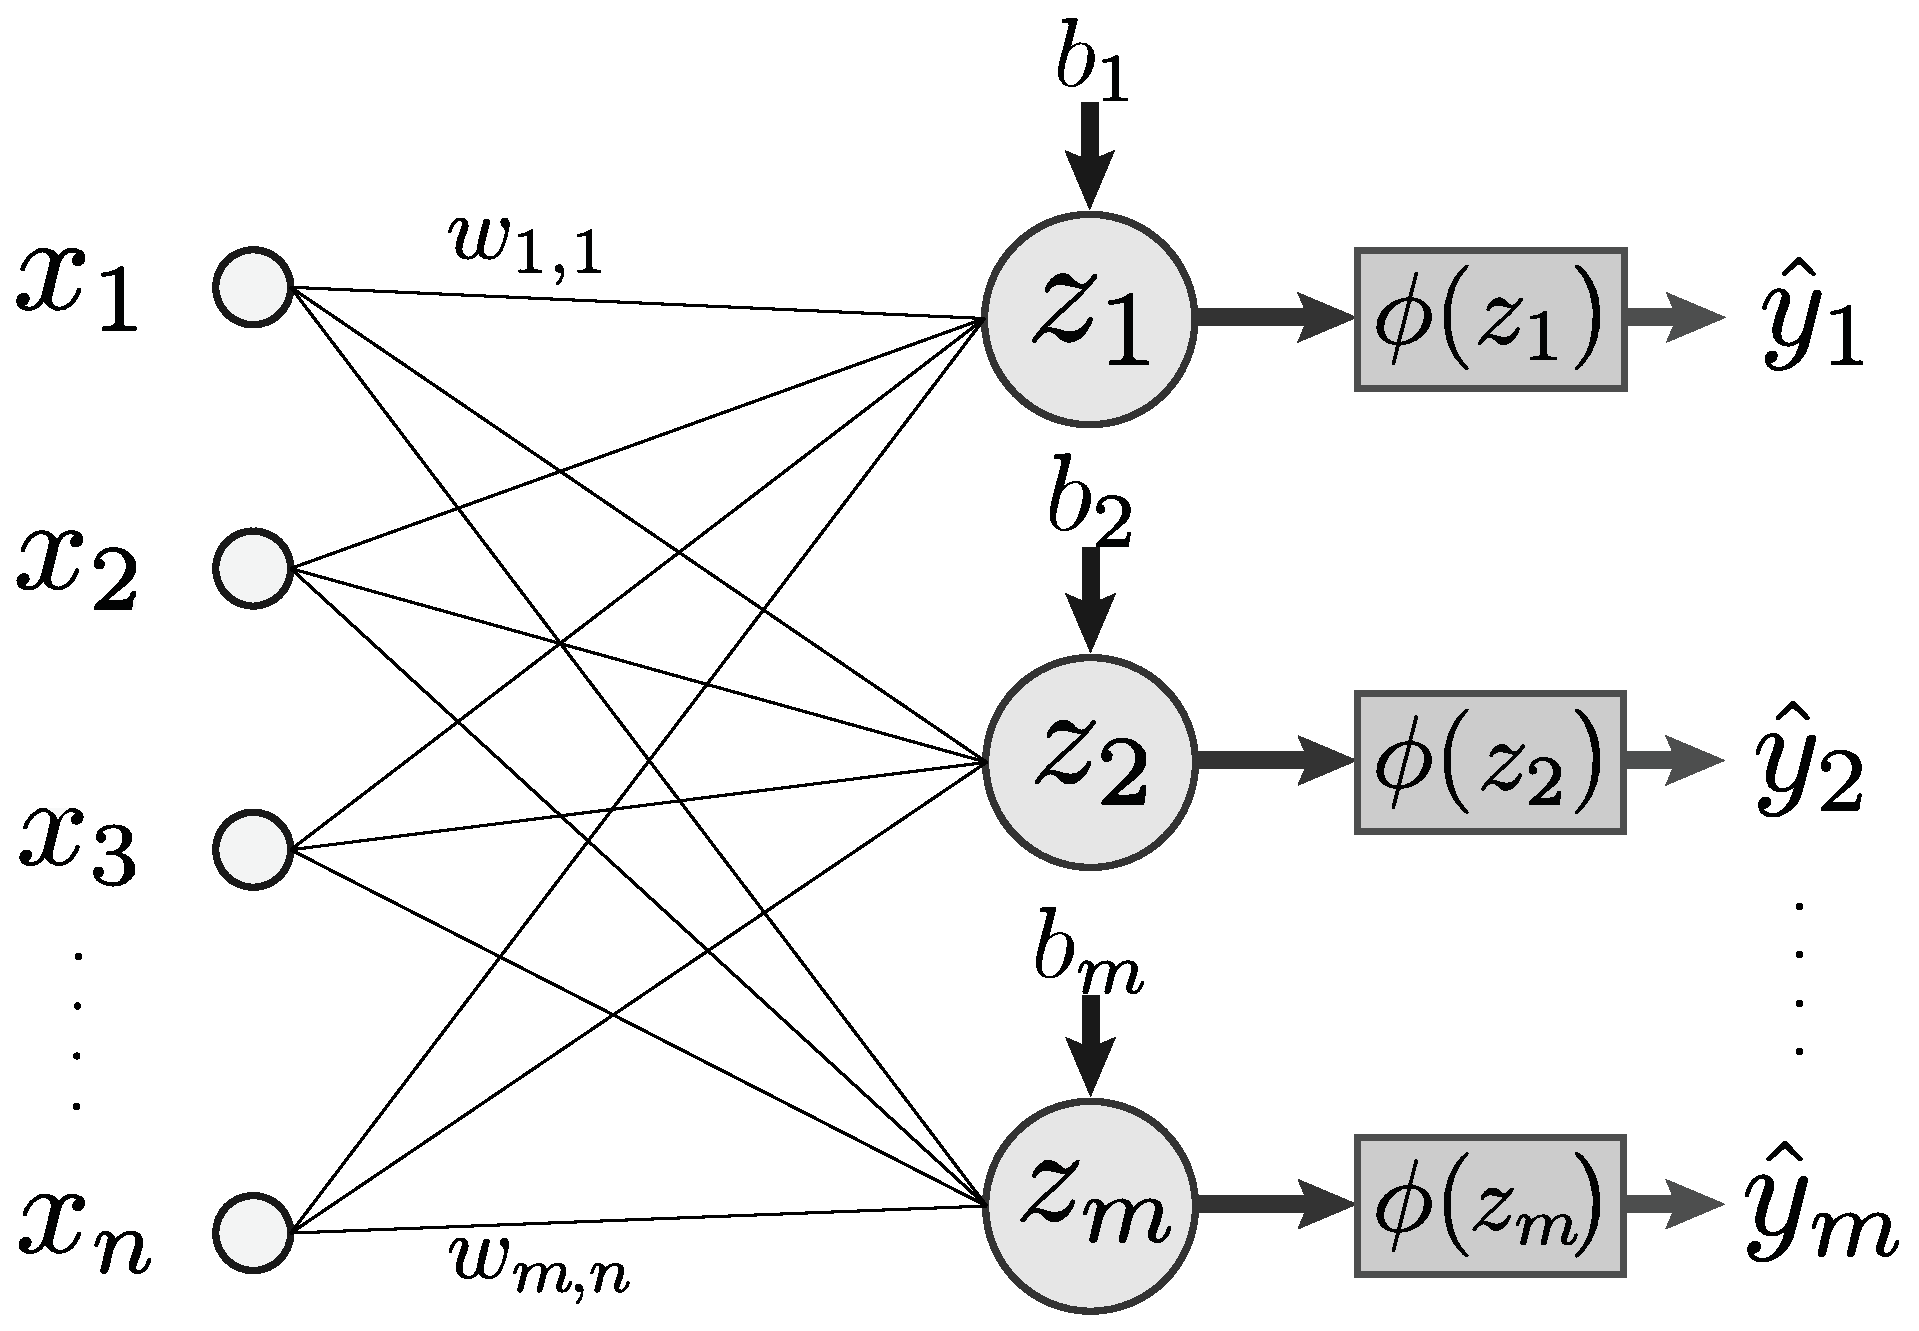
\includegraphics[width=0.7\textwidth]{pics/Figures/ANN.eps}
	\caption{\small{Artificial Neural Network Model \emph{(Single Layer)}}}
	\label{fig:ANN}
	\end{figure}

	The \emph{multi-perceptron, single layer, output} can be computed as:
	\begin{equation}\label{y_hat}
		\bm{\hat{y}} = \phi(\bm{b}+ W\bm{x})
	\end{equation}
	So far, this has been a \textbf{feed-forward} neural network without any kind of \emph{learning}, for the network to start learning there must be a \emph{weight update} algorithm which updates the weights regularly after every entry. This algorithm is known as \emph{Backpropagation} \cite{backprop}, and the formula can be seen in \emph{Equation \ref{backprop}} below: 
	\begin{equation}\label{backprop}
		W^{t+1} = W^{t} - \eta\dfrac{E}{\Delta{W}}
	\end{equation}
	where $W^{t}$ denotes the weight at iteration $t$ of the gradient descent and $\eta$ is a \emph{cost function}.\\[5mm]
	\textbf{Cost functions}, also technically known as \textbf{Loss functions}, vary depending on the faced problem and the desired output of the neural network, for instance, a \emph{Regression} problem will most likely use a \textbf{Mean Absolute Error (MAE)}\cite{qi2020mean} as a cost function which can be computed as:
	\begin{equation}\label{MAE}
		MAE = \dfrac{\sum_{1}^{n}|y_i-x_i|}{n}
	\end{equation}
	where $y_i$ is the predicted value, $x_i$ being the true value and $n$ the total number of data points. However, an \emph{Image Classification} problem will most likely use \textbf{Categorical Crossentropy}\cite{ho2019real} which quantifies the difference between probability distributions in a a multi-class classification problem and it can be computed as:
	\begin{equation}\label{crossentro}
		E = \dfrac{-(\sum_{1}^{N}y_i\log(x_i))}{N}
	\end{equation}
	where $y_i$ is the predicted value, $x_i$ being the true value and $N$ the number of classes.

	
	\subsubsection{Multilayer Perceptrons}\label{MLP}
	\emph{Multilayer Perceptrons (MLPs)} is one class of the \emph{feedfowrard ANNs} where, at least, one \textbf{hidden layer} is present between the input layer and the output layer, a demonstrative diagram can be seen in \emph{Figure~\ref{fig:MLP}}, the hidden layers act like a \emph{black box} where the objective of this so called black box is to extract features from the input, the \emph{deeper} the network, the more features it will be able to extract. But having a \emph{Deep Neural Network (DNN)} could be troubling sometimes as there would be more than 2-3 layers which, in coherence to the more feature extraction, it also acts in a much more complex way which applies a lot of constraints in areas such as software and hardware. The reason for the software constraint with \emph{DNN} is that it will require more data to learn unlike shallower models. As for hardware constraints, the process that is responsible for training \emph{DNNs} is known as \emph{Deep Learning}, Deep Learning requires advanced \emph{GPUs} which could get costly for a user, the essence of a GPU is crucial due to the time constraint that might be present in the absence of a GPU \cite{GPU}. \\[5mm]
	The \emph{black box} could be seen also in \emph{Figure~\ref{fig:MLP}} as a light gray box captioned \emph{Hidden Layers}. 
	
	\begin{figure}[h]
		\centering
		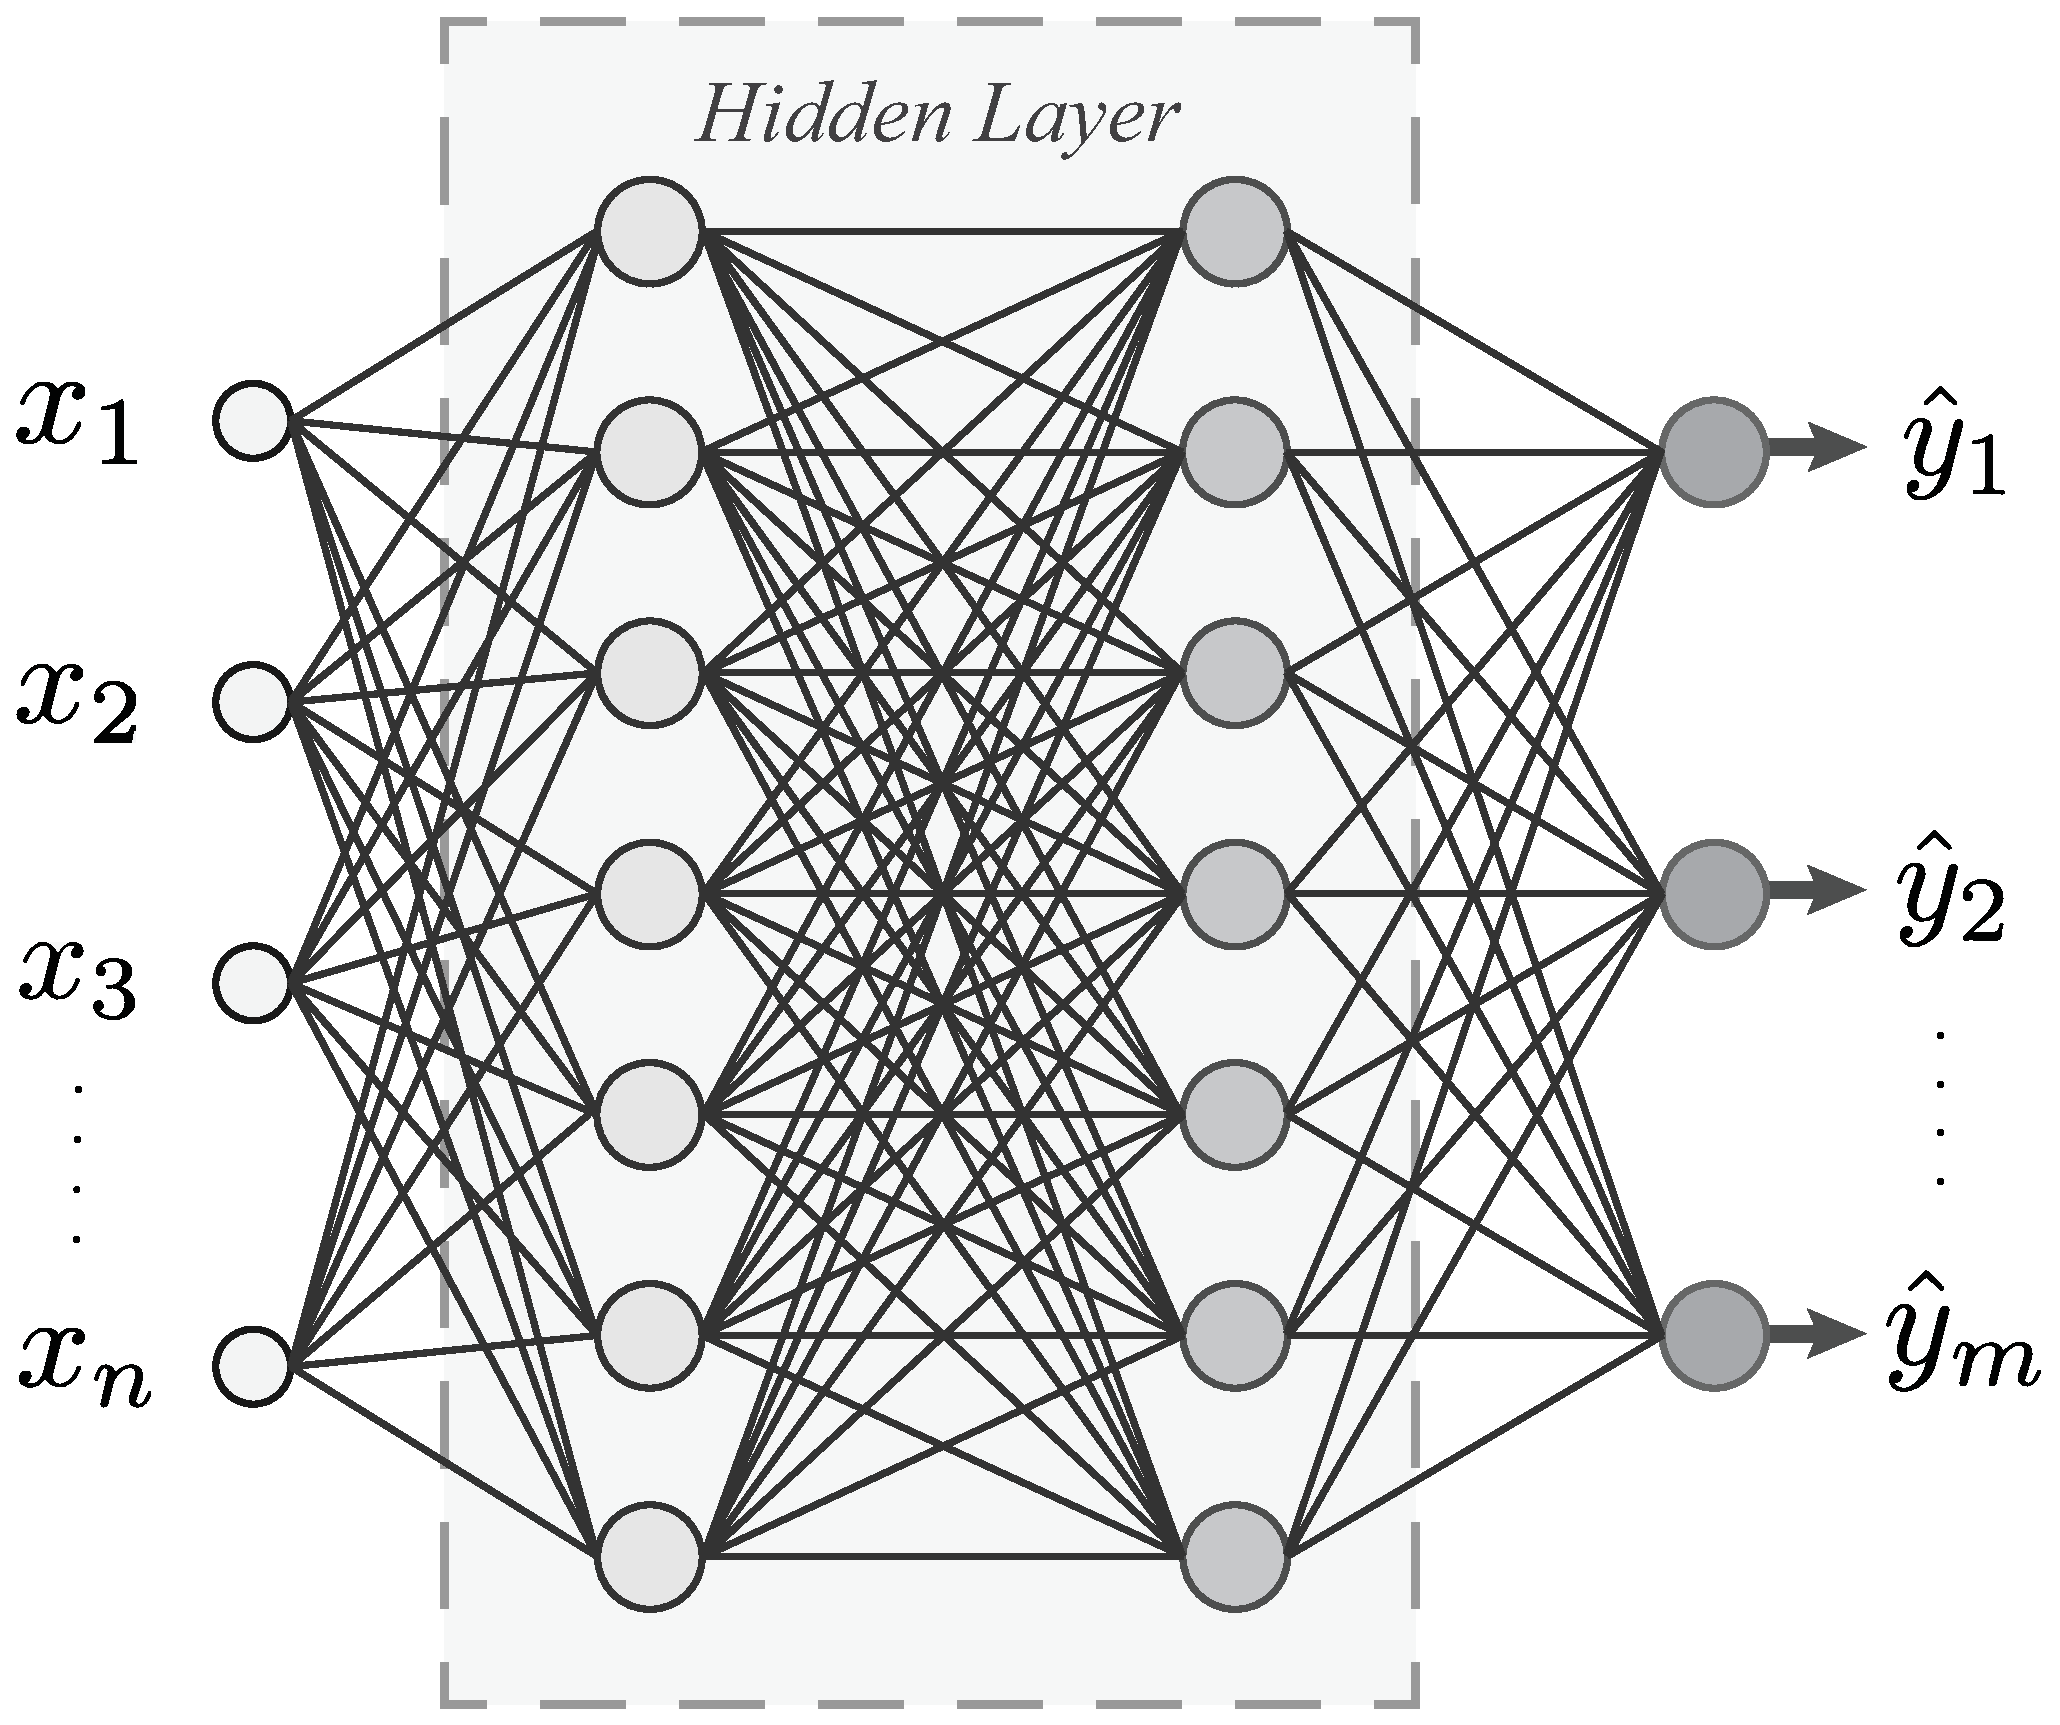
\includegraphics[width=0.7\textwidth]{pics/Figures/MLP.eps}
		\caption{\small{Three layer feedforward network}}
		\label{fig:MLP}
	\end{figure}
	
	However, each layer, of these hidden layers, is still computed as \emph{Equation~\ref{y_hat}}. Bare in mind that the input of the next layer would be the previous layer's computed $\bm{\hat{y}}$, using \emph{Equation~\ref{y_hat}} for the first layer and computing the output layer number $\bm{i}$ as:
	\begin{equation}\label{ANN_y_hat}
		^{(i)}\bm{\hat{y}} = \hspace{1mm} ^{(i)}\phi(^{(i)}\bm{b}+ ^{(i)}W^{(i-1)}\bm{\hat{y}})
	\end{equation}
	\emph{where $\bm{i \geq 2}$}\\
	Moreover, layers where each perceptron is connected to every perceptron of the following layer, as seen in \emph{Figure~\ref{fig:MLP}}, are called \emph{dense} or \emph{fully connected} (FC) layers.
	
	\subsubsection{Convolutional Neural Networks}\label{CNN}	
	\emph{Section~\ref{MLP}} included an explanation on \emph{ANNs} and how it helps in learning more complex functions using deeper networks, however image inputs are not suitable for \emph{MLPs}, since \emph{MLP} networks handle vector inputs, hence requiring the image to be flattened leading to an extreme increase in number of trainable parameters. In other words, using an image of size (512x512) as an input to extract the features would lead to a single perceptron containing \textbf{262.144} trainable parameters (excluding bias) and increasing number of perceptrons in the first hidden layer to around 100, which is not convenient for the size of the image but just setting it as an example, would set the number of trainable parameters to an astonishing \textbf{26.214.400} just for the first layer. In addition, increasing the resolution of the image and using a three-channel \emph{RGB} image will also exceedingly increase the trainable parameters. Therefore, a different kind of architecture is needed to handle images, and that new architecture is called \emph{Convolutional Neural Network (CNN)}.\\[5mm]
	As stated in \cite{DL}, ”Convolutional networks are simply neural networks that use convolution in place of general matrix multiplication in at least one of their layers”. For an input image $I$ and kernel (filter) $K$ , the discrete convolution operation is defined as \cite{DL}:

	\begin{equation}\label{conv}
		c_{i,j} = (I*K)_{i,j} = \sum_{m}\sum_{n}I_{m,n}K_{i-m,j-n}
	\end{equation}
	In general the convolution operation on these images would produce an output feature image which is produced by convolving the input image with the kernel, the kernel would be a set of weights (trainable parameters) which the size could be defined by a user.\\[5mm]
	Although many implementations talk about convolution and applying \emph{Equation~\ref{conv}} to the "\emph{Convolutional} Neural Network", an alternative method is used which is called \emph{cross-correlation}. As we can see in \emph{Equation~\ref{conv}}, where $m$ and $n$ iterate over valid subscripts of both $I_{m,n}$ and $K_{i-m,j-n}$, the \emph{filter} $K$ is flipped thus producing a \textbf{flipped} output, since the filter would be sliding in the negative direction. Consequently, an alternative variant is introduced called \emph{cross-correlation} and it is computed as follows:
	\begin{equation}\label{cross-corr}
		c_{i,j} = (I*K)_{i,j} = \sum_{m}\sum_{n}I_{i+m,j+n}K_{i,j}
	\end{equation}
	Hence producing an output which is not flipped as seen in \emph{Figure~\ref{fig:cross-corr}}. 
	
	\begin{figure}[h]
		\centering
		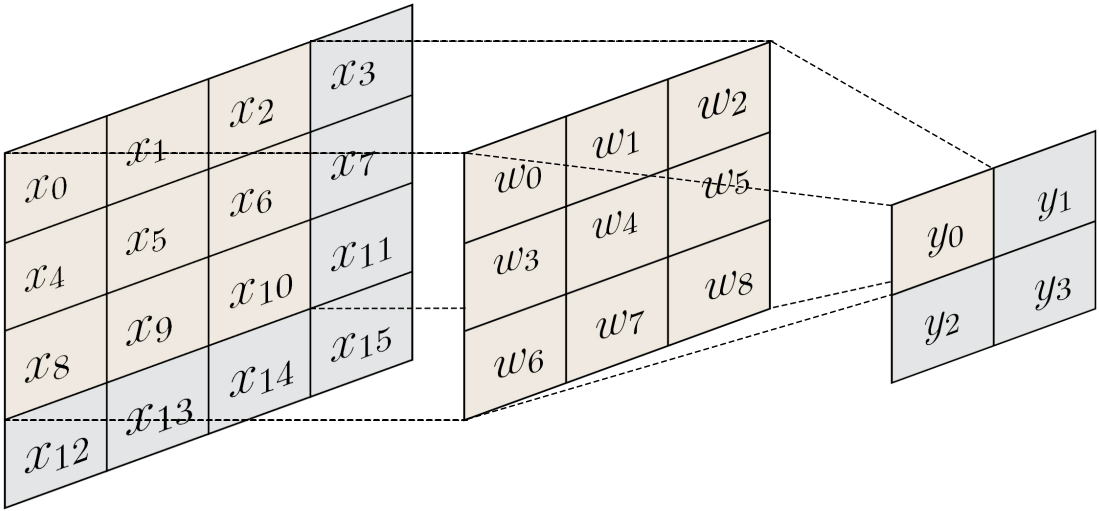
\includegraphics[width=0.8\textwidth]{pics/Figures/convolution.png}
		\caption{\small{An illustration of \emph{Cross-Correlation}}}
		\label{fig:cross-corr}
	\end{figure}
	The process can be seen as the summation of the element-wise product between the kernel and any spatial location of center $(i, j)$, then moving the kernel by the amount of \emph{stride }to another location until the whole image is covered. Additionally, for multi-channel input image the \emph{Equation~\ref{cross-corr}} can be expanded as follows:
	\begin{equation}
		c_{i,j} = (I*K)_{i,j} = \sum_{m}\sum_{n}\sum{d}I_{i+m,j+n,d}K_{i,j,d}
	\end{equation}
	where d iterates over valid subscripts of both $I_{i+m,j+n,d}$ and $K_{i,j,d}$. Note it is frequent to add bias to the equation. Multiple kernels can be applied to the same input image to obtain several feature maps. Thus, the output depth is equal to number of kernels / filters applied. One of the characteristics of a convolutional layer is \textbf{parameter sharing}; it is possible to assume that if a specific filter is useful in some region, then it is useful in other regions as well. Under this assumption, the parameters are shared along the depth \cite{par_share} reducing the number of learnable parameters. Moreover, it is frequent to apply an activation function to feature maps in order to obtain activation maps.
\\[5mm]
	Convolution reduces the size of the input image. For this reason, when several convolution layers are used, the image size decreases drastically. As a counter-measurement, an outer frame is added to the image, limiting the size reduction. This process is called \textbf{padding}. It is common to use zeros as values for the frame and this is called \emph{zero padding}, while reflecting values of rows and columns into the frame is named \emph{reflection padding}.\\[5mm]
	For an image of height $(H_i)$ and width $(W_i)$, the size of the image post convolution is computed as:
	\begin{equation}\label{width}
		\hat{W}_i = \dfrac{W_i-k+2P_i}{s}+1
	\end{equation}
	\begin{equation}\label{height}
		\hat{H}_i = \dfrac{H_i-k+2P_i}{s}+1
	\end{equation}

	where $\hat{W}_i$ and $\hat{H}_i$ are the new width and height, respectivelt, of post convolution process. $k$ is the kernel size, $s$ being the stride and the padding size denoted as $P_i$. 
	
	\begin{figure}[h]
		\centering
		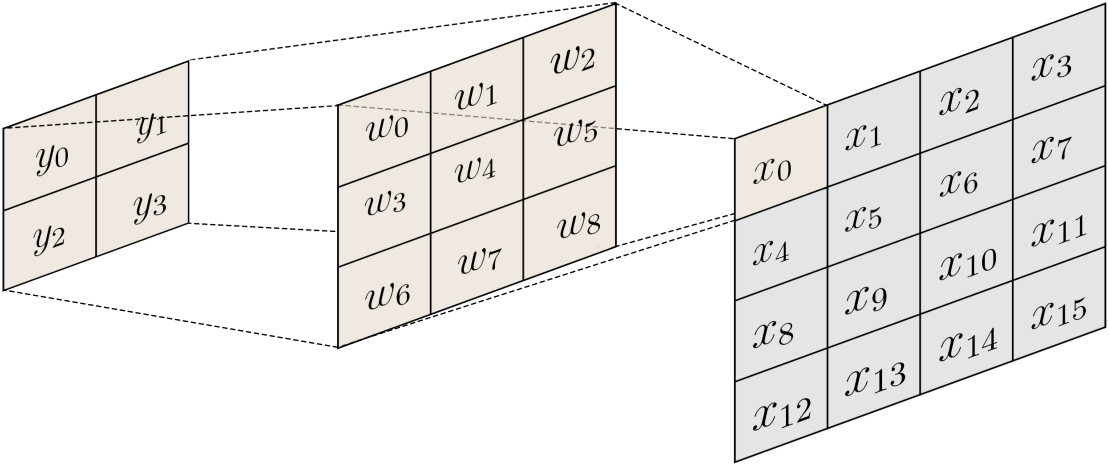
\includegraphics[width=0.8\textwidth]{pics/Figures/reverse_convolution.png}
		\caption{\small{An illustration of \emph{Transposed Convolution}}}
		\label{fig:T_Conv}
	\end{figure}
	
	In a convolutional layer, the kernel defines a convolution that has a forward pass and backward pass. Flipping the passes would result in \emph{Transposed Convolution} or known as \emph{fractionally strided convolution} \cite{stride}, which is used for upsampling. Transposed Convolution can as well be visualized in \emph{Figure~\ref{fig:T_Conv}}.
	\subsection{Computer Vision}\label{CV}
	\emph{Human vision} is similar to \emph{Computer Vision (CV)}, with the exception that people have a head start. Human vision benefits from lifetimes of context to teach it how to distinguish objects apart, how far away they are, whether they are moving, and whether something is incorrect with an image. CV teaches computers to execute similar tasks, but using cameras, data, and algorithms rather than retinas, optic nerves, and a visual cortex, it must do it in a \textbf{fraction of the time}. Because a system trained to check items or monitor a production asset can assess hundreds of products or processes per minute, detecting faults or issues that are invisible to humans, it can swiftly \textbf{outperform humans}. The speed and the methods will be discussed in \emph{Section~\ref{Classification}} and \emph{Section~\ref{Obj Detection}}.
	\subsubsection{Image Classification}\label{Classification}
	Some text about \textbf{Image Classification}
	\begin{figure}[h]
		\centering
		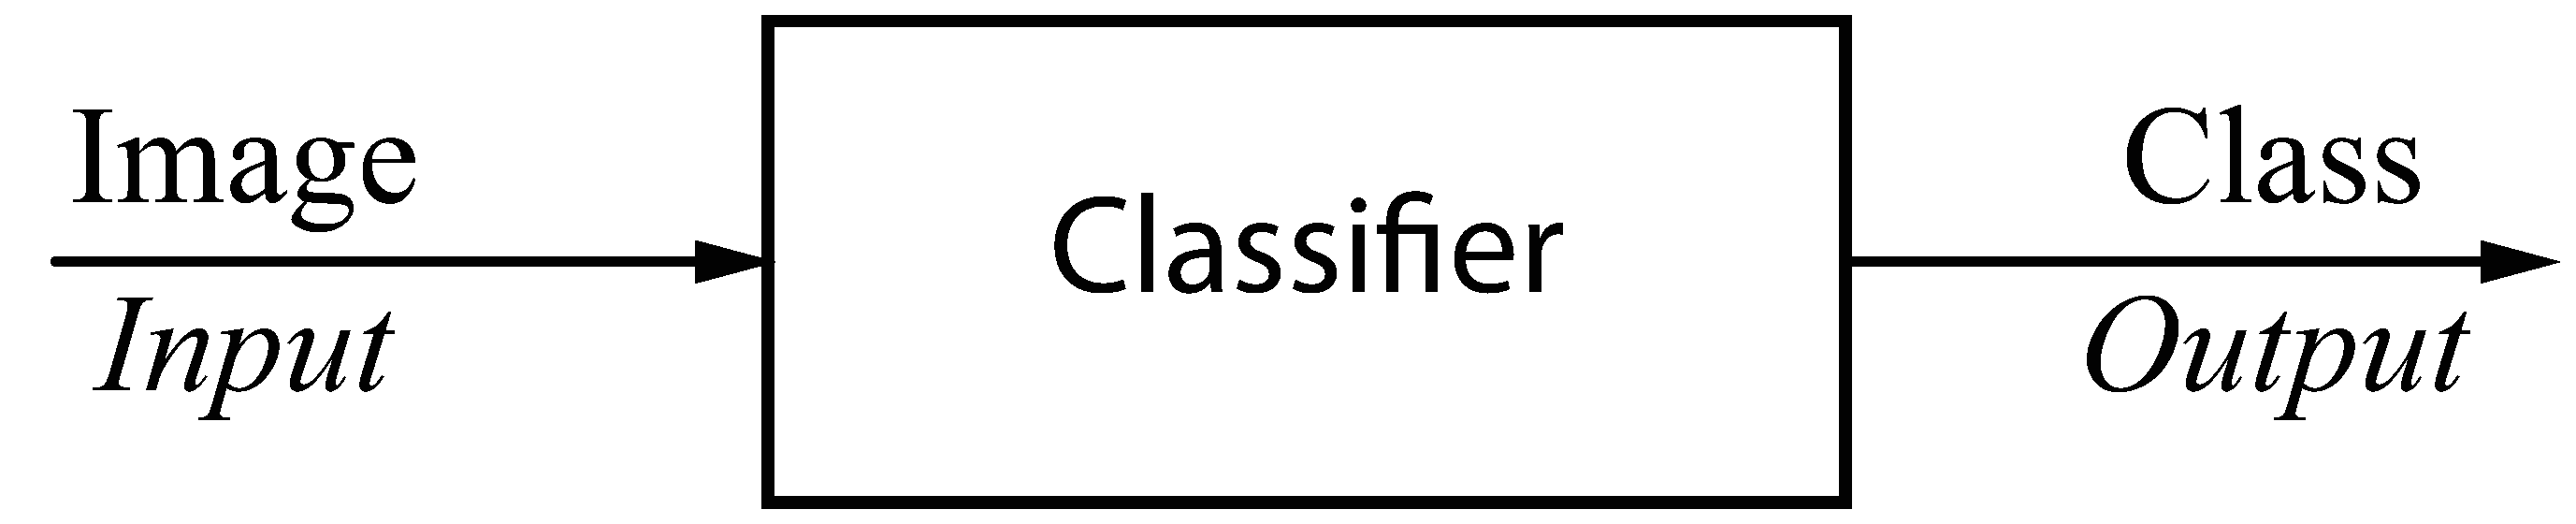
\includegraphics[width=0.5\textwidth]{pics/Figures/Classifier_Block_Diagram.eps}
		\caption{\small{Classifier Diagram}}
		\label{fig:Classifier}
	\end{figure}
	\subsubsection{Object Detection}\label{Obj Detection}
	In an object detection task, a model has to both classify objects / instances appearing in an image and localize them within the image. The localization is represented by a 2D bounding box, in which the structure of the object detector is visible in \emph{Figure~\ref{fig:Obj Detector}}. State of the art networks tackling this task are divided into two main groups. The first group are the single stage object detection network, which prioritize the \textbf{inference speed} over than the accuracy. Single stage methods include \emph{YOLO} \cite{Objdet2} and \emph{RetinaNet} \cite{Retina}.The second group of methods is the two stage methods, which are tuned for \textbf{accuracy} over inference speed. An example of two stage methods is the Faster R-CNN \cite{Objdet}.
	\begin{figure}[h]
		\centering
		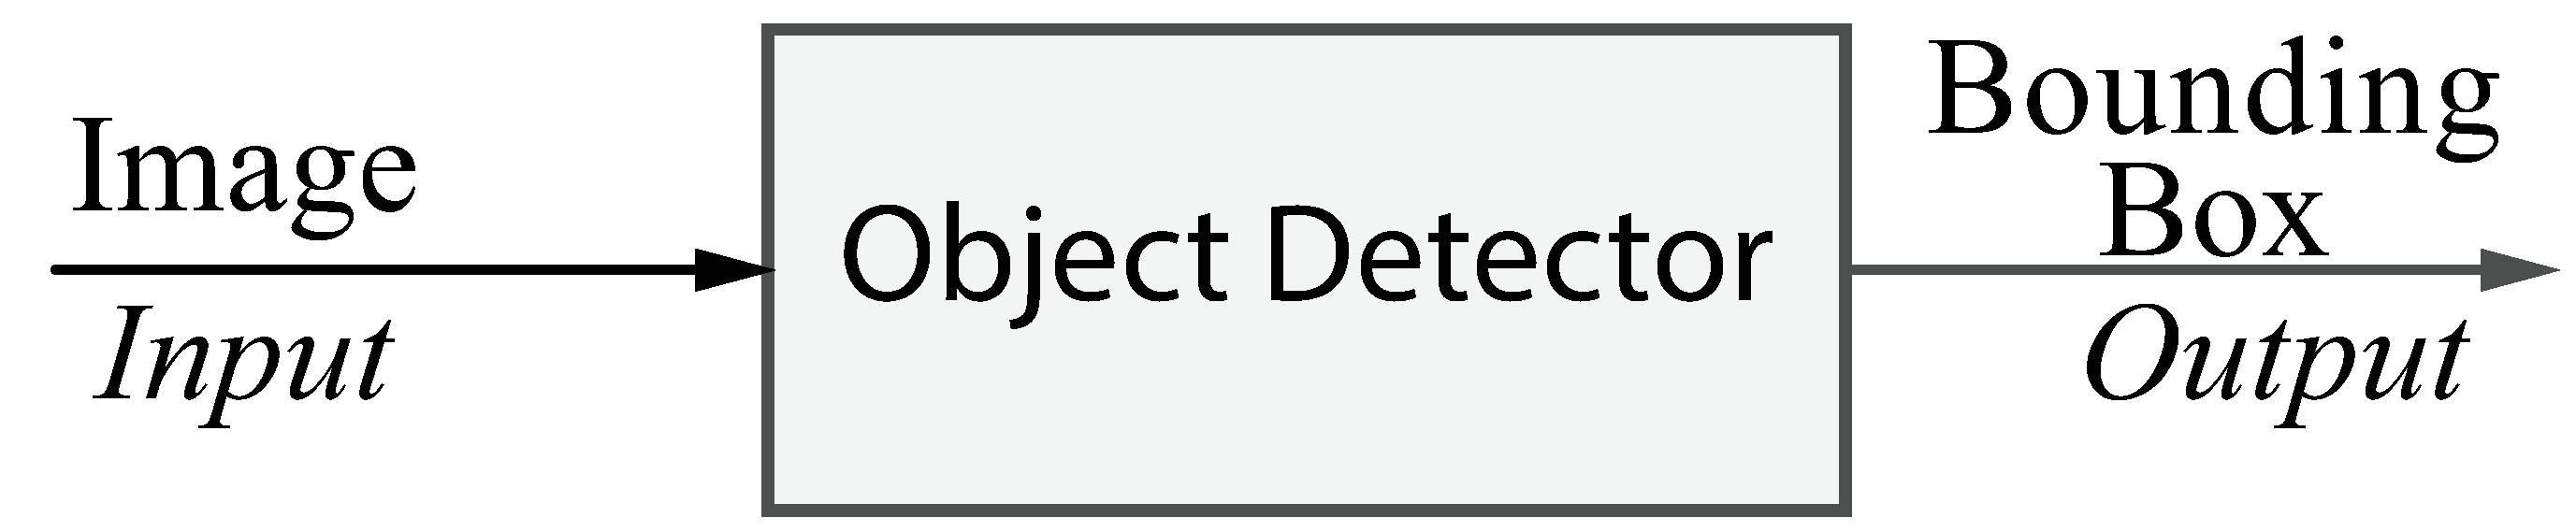
\includegraphics[width=0.5\textwidth]{pics/Figures/Obj_Det_Block_Diagram.eps}
		\caption{\small{Object Detection Diagram}}
		\label{fig:Obj Detector}
	\end{figure}
	
	\subsection{Hierarchy Classifier}
	An explanation on the Hierarchical approach.
	\begin{figure}[h]
		\centering
		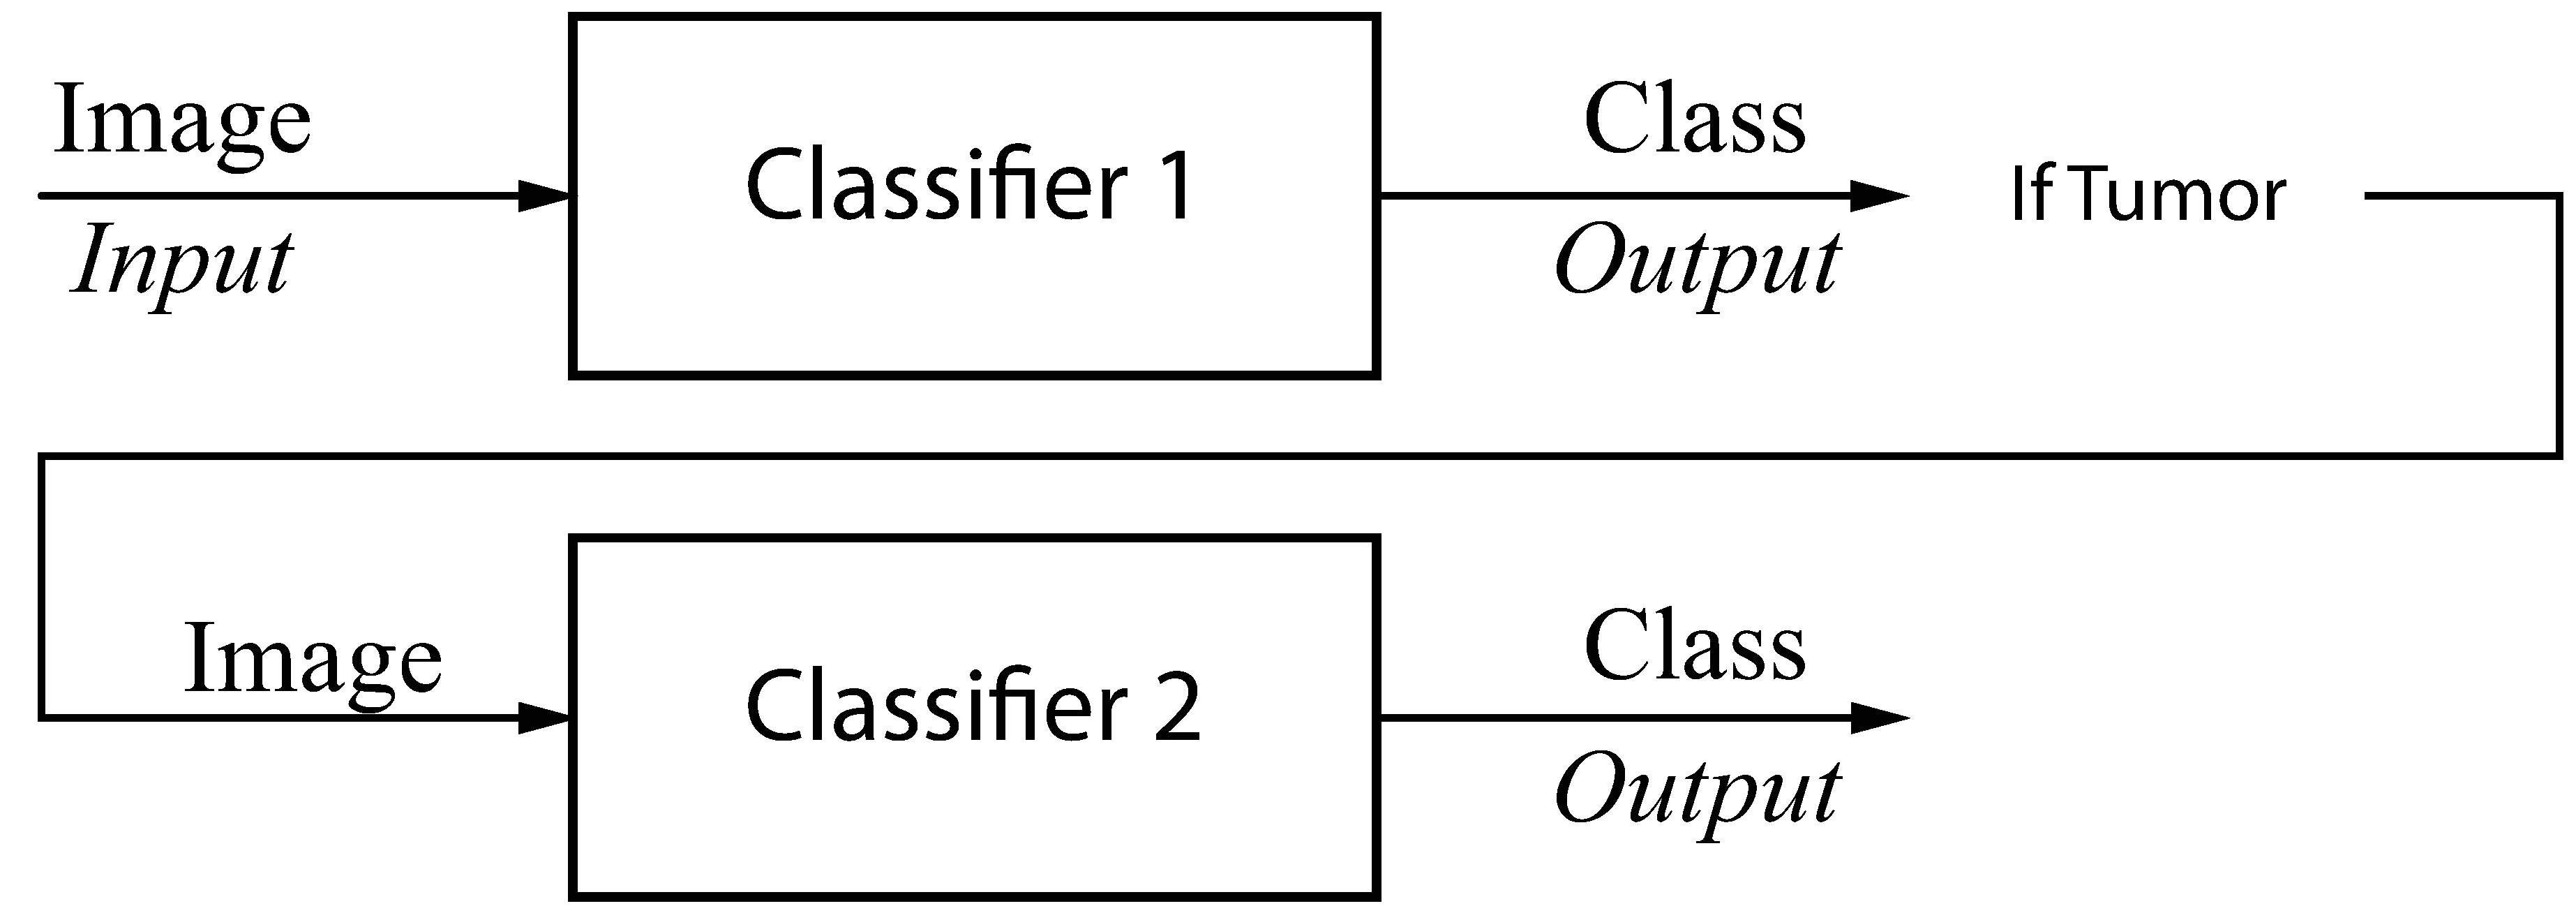
\includegraphics[width=0.5\textwidth]{pics/Figures/Hierarchical_Classifier_Block_Diagram.eps}
		\caption{\small{Hierarchical Classifier Diagram}}
		\label{fig:Hierarchical Classifier}
	\end{figure}
	some basic explanation on \emph{Figure \ref{fig:Hierarchical Classifier}} which is a normal approach found in /ref{GJU paper}.
	\newpage
	
	
	\section{Hierarchical Method}\label{Meth}
	
	\begin{figure}[h]
		\centering
		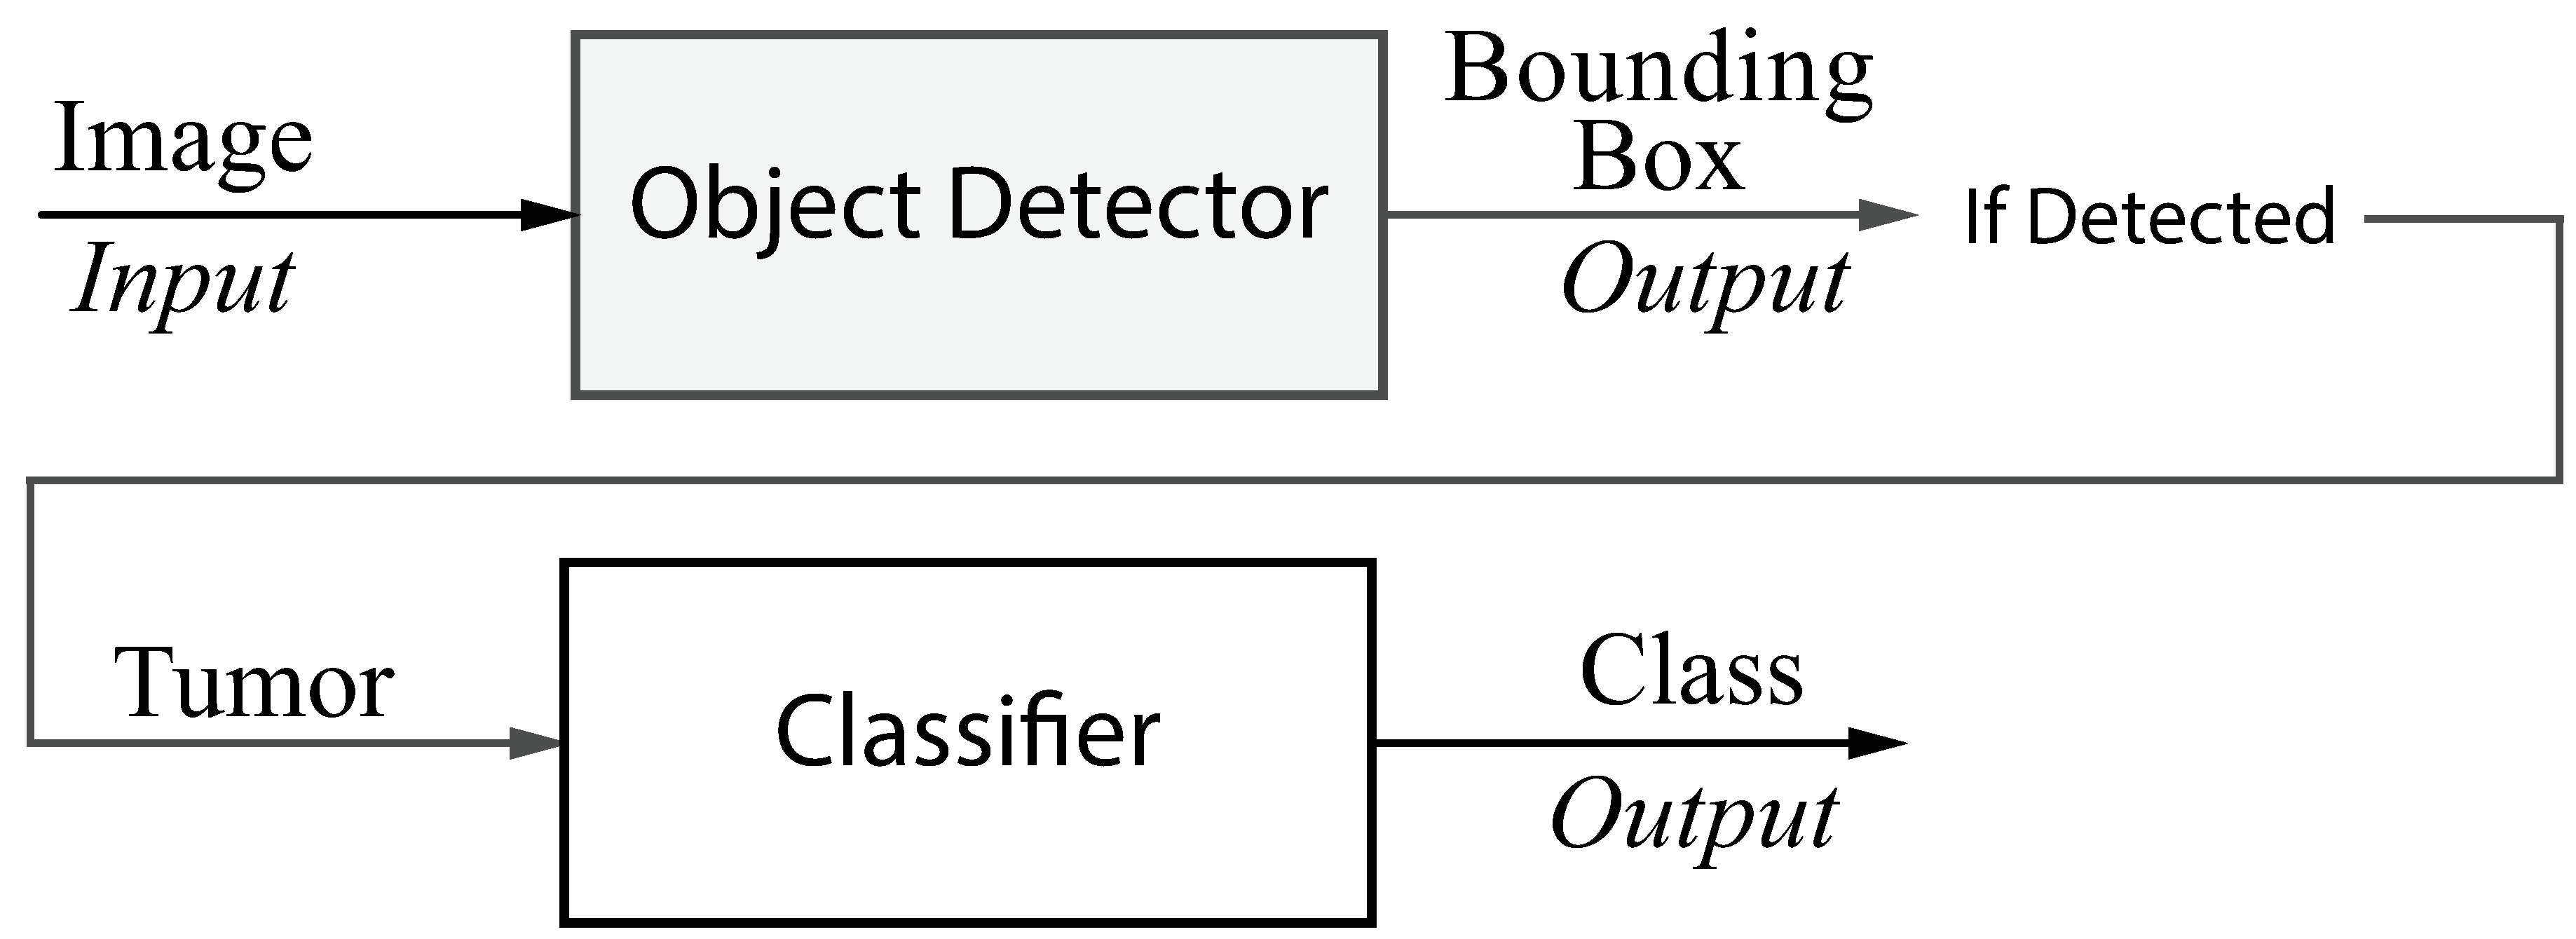
\includegraphics[width=0.5\textwidth]{pics/Figures/Hierarchical_Obj_Det_Block_Diagram.eps}
		\caption{\small{Object Detection Diagram}}
		\label{fig:Hierarchical Obj Detector}
	\end{figure}
	some in depth explanation on \emph{Figure \ref{fig:Hierarchical Obj Detector}} alongside many more figures to explain the thought process 
	\subsection{Dataset}\label{Data}
	
	Choosing a dataset for this problem is crucial to many stages, first and foremost is the \emph{quality of the data}. Does the data clearly portray the goal that should be acquired? Secondly is the \emph{quantity of the dataset}, just like the quality, quantity is as important. \textbf{Neural Networks} require a lot of data, but the quantity mainly depends on the following:
	\begin{itemize}
		\item features that must be extracted from the data
		\item type of Neural Network
		\item data quality
		\item the desired goal
	\end{itemize}
	With that being said, the data is a vital part of this project, and to be able to achieve high accuracy and precision of detecting the cancerous cells, it is a must to obtain high grade dataset. 
	The most common age for the diagnosis of breast cancer is \emph{over 50} years of age. This has been conducted by the National Cancer Institute that the median age of breast cancer patients is between the age of \emph{55} to \emph{64} \cite{CDC}. 
	\\[5mm]
	
	
	\begin{figure}[h]
		\centering
		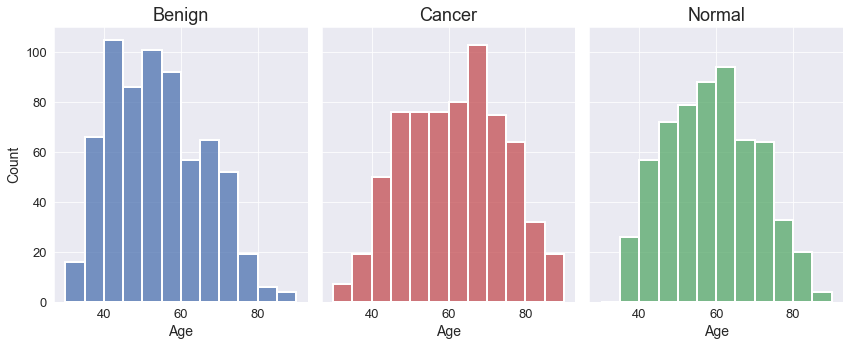
\includegraphics[width=1\textwidth]{pics/Figures/Age_Dist.png}
		\caption{\small{Age Distribution}}
		\label{fig:Age_Dist}
	\end{figure}
	\begin{figure}[h]
		\centering
		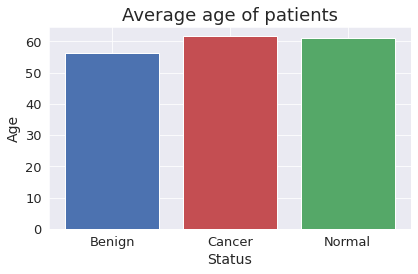
\includegraphics[width=0.5\textwidth]{pics/Figures/Avg_Age.png}
		\caption{\small{Average Age}}
		\label{fig:Avg_Age}
	\end{figure}
	
	\newpage	
	\section{Conclusion}
	Conclusion goes here
	\newpage

	\bibliographystyle{IEEEtran}
	\bibliography{IEEEabrv,myrefs}
	
	
\end{document}

\newpage
\setstretch{1}  %reduce bibliography line spacing
\end{document}